\documentclass{article} \usepackage[textwidth=18cm,textheight=18cm]{geometry}

\title{Git} \date{\vspace{-5ex}} \author{Stefano Entatti}
\usepackage{hyperref}
\usepackage{graphicx}
\setlength{\parindent}{10pt}

\begin{document}

\maketitle

\newcommand{\code}[1]{\texttt{#1}}

\section{Cos'è un sistema di controllo di versione}

Nella realizzazione di un progetto software potresti esserti accorto di voler
tenere traccia dei tuoi progressi, magari registrandoli in modo da sapere cosa
hai fatto e quando, o di voler tornare al momento esattamente prima a quella
modifica che non fa funzionare più nulla. 

Potresti provare, ogni volta che apporti modifiche importanti, a creare una
nuova copia del progetto, numerarla e magari annotarti quali cambiamenti ha
portato. Man mano che il progetto avanza, le copie possono diventare moltissime
e serve comunque confrontare i file riga per riga per capire cosa cambia da una
copia all'altra.

Se al progetto lavorano più persone, (e quindi carichi il progetto su drive) non
è comunque possibile che più persone modifichino il codice nello stesso momento,
e se ognuno modifica una copia diversa, queste vanno poi unite sempre a mano con
dei copia e incolla.

Un sistema di controllo di versione tiene traccia di tutte le modifiche
effettuate su un insieme di file (che compongono il progetto), ovvero di chi le
ha fatte, quando, quali righe sono state tolte e quali aggiunte. Ogni registrazione
di modifica riporta l'autore, un titolo e una descrizione che spiega in dettaglio
il perchè e stata necessaria o qualche peculiarità della modifica stessa
in modo da facilitare la comprensione ad altri sviluppatore o ad una rilettura
in futuro. Inoltre in questo modo è possibile navigare e riportarsi in 
qualsiasi punto della storia del progetto.

Per permettere a più persone di lavorare nello stesso momento ognuno
copia in locale il progetto da un punto di riferimento (server comune ad
esempio), e dopo aver apportato le modifiche necessarie è possibile unirle 
tenendo traccia di chi ha modificato cosa ed in quale ordine.

Esistono molti software di controllo versione, tra i più famosi ci sono Git,
CVS, Subversion, Mercurial, Bazaar e BitKeeper.

\section{Il sistema di controllo versione Git}

Git è il sistema di controllo versione più utilizzato, ed è anche uno dei più
semplici da usare. é nato nel 2005 ed è stato ideato da Linus Torvalds (il
creatore di Linux) per facilitare lo sviluppo del kernel di Linux, uno dei
progetti opensource più grandi, a cui lavorano moltissime persone. Anche git è
opensource.

Git è distribuito, ciò significa che l'intero \textbf{repository}, ovvero
tutti i file che compongono un progetto, tra cui sorgenti, readme e file creati
da git per tenere traccia dello storico delle modifiche può essere memorizzato
su un server a cui possono accedere tutti i membri del progetto. Allo stesso
tempo ognuno può tenere una copia completa del del repository in locale e
utilizzare tutte le funzionalità di git anche \textbf{offline}. L'interazione col server
è limiata a quando lo sviluppatore desidera scaricare le modifiche effettuate da
altri o vuole caricare le proprie sul server.

Git è nato come un programma a riga di comando, e anche se viene considerato più
efficiente se utilizzato in questo modo, oggi esistono molti client grafici e
estensioni che permettono di usufruire della maggior parte delle funzionalità di
git direttamente dall'IDE.

\section{Branching}

Git è in grado di gestire contemporaneamente più sviluppi all'interno della
stessa copia del progetto, questi si chiamano \textbf{branch}. Con più sviluppi si 
intendono più tipologie di modifiche differenti anche all'interno dello stesso file.
Si può saltare da uno sviluppo all'altro senza perdere nessuna modifica
evitando di avere più copie del progetto.

Ogni repository git possiede almeno un branch, chiamato \textbf{master}.
Possono essere creati infiniti branch, ognuno dei quali può essere utilizzato
per la realizzazione di una particolare funzionalita', in modo che modifiche su parti
molto diverse del codice non possano causare conflitti. Spesso un singolo
sviluppatore lavora su un proprio branch, in modo da non dover gestire anche i
cambiamenti fatti da altri mentre svolge il suo compito. 

Oppure il branch master può essere quello che viene distribuito agli
utilizzatori del software perchè considerato stabile, mentre gli altri possono
essere sperimentali e dunque contenere bug o modifiche che possono essere 
scartate senza compromettere tutto il resto. 

A volte vari branch servono a separare versioni
con funzionalità leggermente diverse dello stesso software.

Un branch viene creato a partire da un altro. Dopo la creazione di un branch
``figlio'' le modifiche che nel tempo vengono apportate su questo rimangono
completamente separate da quelle che eventualmente continuano ad essere
apportate sul ``padre''. Se vengono creati più branch, almeno uno di questi discende
da master.

Ovviamente, due branch possono essere uniti tramite un \textbf{merge}. Gli
algoritmi di merge confrontano due branch riga per riga, manentendo quella
appartenente al branch in cui è stata modificata. Se però la stessa riga è stata
cambiata in entrambi i branch si crea un conflitto e git richiede all'utente di 
risolverlo a mano.

Si può passare in qualsiasi momento da un branch all'altro.

\section{Comandi principali}

Git offre moltissimi comandi, ognuno dei quali svolge un piccolo insieme di
funzionalità. Ogni comando (in questa sezione tratteremo i principali) è sempre preceduto da
``git''. Ognuno può accettare un diverso numero di argomenti e di opzioni
(tratteremo le principali per ogni comando), spesso precedute da un singolo o da
un doppio meno. 

\subsection{init, clone}

Per creare un nuovo repository locale si utilizza init (stando all'interno
della cartella del progetto del quale si vuole tenere traccia):

\begin{verbatim}
$ git init prova
Inizializzato repository Git vuoto in /home/user/prova/.git/
\end{verbatim}

Per copiare un intero repository remoto si utilizza git clone. Viene scaricato
solo il branch master, ma una volta clonato si può accedere a tutti gli altri

\begin{verbatim}
$ git clone https://github.com/torvalds/linux.git
\end{verbatim}

Per utilizzare tutti gli altri comandi, occorre posizionarsi all' interno della
cartella del repository, che viene creata in automatico da clone e init.

\subsection{Commit}

Ogni volta che si fa una certa quantità di cambiamenti è utile fare un commit,
ovvero segnare un punto nello sviluppo a cui sarà sempre possibile tornare,
quindi registrare e descrivere queste modifiche. 

\begin{verbatim}
$ git commit
\end{verbatim}

Questo comando aprirà l'editor di default di git. Nella prima riga va scritto il
titolo del commit. è una buona norma che il titolo mantenga una lunghezza
massima di 72 caratteri e contenga solo nomi e verbi al presente. La seconda si
lascia sempre vuota e dalla terza inizia la descrizione, che può essere
molto lunga e dettagliata per spiegare in modo discorsivo cosa si è fatto, 
perché e se eventualmente ha causato dei problemi.

\begin{figure}
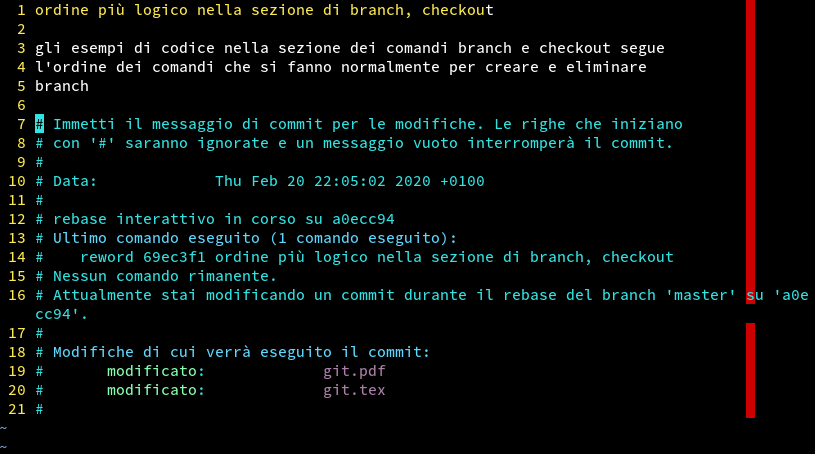
\includegraphics[width=6in]{vimEditCommit.png}
\centering
\caption{scrittura del testo di un commit in vim}
\end{figure}

se non si necessita di una descrizione si può utilizzare l'opzione -m
(``message''):

\begin{verbatim}
$ git commit -m "add options page"
\end{verbatim}

Ci sono varie teorie  sulla lunghezza e il contenuto dei messaggi e delle
descrizioni dei commit e su \emph{ogni quanto} si debba committare. In genere un
commit deve essere relativo ad un solo argomento e non comprendere modifiche
totalmente indipendenti tra di loro. I messaggi di commit non devono essere
generici (come ``fix crash'') altrimenti col passare del tempo sarà impossibile
capire cosa si era fatto senza controlare il codice.

L'opzione -s (``signed'') aggiunge la firma dell'autore nella descrizione:

\begin{verbatim}
Signed-off-by: user1 <user1@gmail.com>
\end{verbatim}

\subsection{Add, rm, reset}

I file coinvolti dal commit devono essere prima selezionati con add. In questo
modo si entra nella \textit{staging area}. è uno stato intermedio che sta prima di
un commit per tracciare le modifiche momentanee in caso di piu' prove.

Se ad esempio si modificano functions.cpp, functions.hpp e main.cpp:

\begin{verbatim}
$ git add functions.cpp functions.hpp
$ git commit -m "added get function"
\end{verbatim}

In questo caso le moficiche di main.cpp non verranno aggiunte al commit \code{added
get function}.

Qualsiasi modifica effettuata su \code{functions.cpp} o \code{functions.hpp} dopo l'utilizzo
di add verrebbe anch'essa esclusa dal commit.

Git add si comporta in modo indifferente sia per file appena creati che per le
modifiche di file già esistenti.

L'opzione -a (``all'') passata al comando di commit include automaticamente tutte
le modifiche attualmente pendenti.

Alcune opzioni utili per add:

\begin{itemize}
    \item \code{-A} aggiunge qualsiasi modifica all'area di staging
    \item \code{.} come -A ma non aggiunge la rimozione dei file
    \item \code{-u} non aggiunge i nuovi file
\end{itemize}

Il comando git rm fa il contrario di add, mentre reset pulisce completamente la
staging area.

\subsection{Push}

Permette di caricare un numero illimitato di commit su un branch di un
repository remoto. Le modifiche locali vengono unite a quelle remote.

Git non permette di effettuare un push se la \textbf{storia}, intesa come sequenza di commit,
del branch remoto non è uguale al branch locale, escludendo i commit
appena aggiunti fatti in locale. Se ci si trova in questa situazione occorre effettuare un riallineamento,
(pull/rebase).

\begin{verbatim}
$ git push
Username for 'https://github.com': Stivvo
Password for 'https://Stivvo@github.com':
To https://github.com/Stivvo/msTest.git
 ! [rejected]        master -> master (fetch first)
error: push di alcuni riferimenti su 'https://github.com/Stivvo/msTest.git' non riuscito
Gli aggiornamenti sono stati rifiutati perché il remoto contiene delle
modifiche che non hai localmente. Ciò solitamente è causato da un push
da un altro repository allo stesso riferimento. Potresti voler integrare
le modifiche remote (ad es. con 'git pull ...') prima di eseguire
nuovamente il push.
Vedi la 'Nota sui fast forward' in 'git push --help' per ulteriori
dettagli
\end{verbatim}

\subsection{Merge, Pull, fetch}

\textbf{Merge} permette di fondere le modifiche di due branch, locali o remoti (o anche
commit diversi dello stesso branch) come ad esempio quando devo unire nel branch principale
le modifiche fatte su un branch per correggere dei bug. Se si effettua un pull come suggerito
sopra, avverrà infatti un merge. Se git rileva dei conflitti segnala all'utente
di risolverli manualmente. 

\textbf{Fetch} permette di aggiornare lo stato dei branch in remoto per controllore
se ci sono branch nuovi o magari nuovi commit sul branch al quale si sta lavorando per evitare
di rimanere disallineati con il repository di riferimento.

\textbf{Pull} è in sostanza un fetch seguito da un merge, ed è quello che capita di
utilzzare più spesso. In generale pull fonde ciò che si trova al momento sul
branch del repository remoto con quello locale.

Pull e fetch chiamati senza argomenti vanno a prelevare la versione remota del
branch su cui si è localmente.

\begin{verbatim}
<<<<<<< HEAD
class FirstClass {
=======
class SecondClass {
>>>>>>> 4ceb8e7c4fe78b59c00be99418f54280df19078c
\end{verbatim}

Questo è il caso in cui mentre il repository locale rimaneva indietro di alcuni
commit la classe è stata rinominata in FirstClass da un primo sviluppatore. Nel
frattempo un secondo ha fatto un push di un commit in cui l'ha chiamata
SecondClass. Quando il primo sviluppatore si trova a dover fare il pull delle modifiche del
secondo, per risovere i conflitti di merge deve scegliere tra la versione locale
(HEAD) e quella dell'altro, identificata dal codice hash (lunga serie di numeri e
caratteri) del commit che ha
rinominato la classe in SecondClass. Il prossimo push sarà quello del commit di
merge, automaticamente creato da git.

\subsection{Checkout, Branch, merge}

Git branch senza opzioni viene utilizzato per creare un nuovo branch locale. La
creazione del branch develop:

\begin{verbatim}
$ git branch develop
\end{verbatim}

Per posizionarsi su develop:

\begin{verbatim}
$ git checkout develop
M	git.pdf
M	git.tex
Si è passati al branch 'develop'
\end{verbatim}

Se si prova a eseguire un push dal branch appena creato occorre
aggiungerlo alla lista dei branch remoti:

\begin{verbatim}
fatal: Il branch corrente develop non ha alcun branch upstream.
Per eseguire il push del branch corrente ed impostare il remoto come upstream, usa

    git push --set-upstream origin develop
\end{verbatim}

L'opzione --all mostra tutti i branch locali e remoti. Il branch seguito
dall'asterisco è quello su cui si è posizionati correntemtente.

\begin{verbatim}
$ git branch --all
* develop
  master
  temp
  remotes/origin/HEAD -> origin/master
  remotes/origin/develop
  remotes/origin/master
\end{verbatim}

In questo caso, temp è solamente locale.

L'opzione -d invece elimina un branch. Non è possibile eliminare il branch corrente:

\begin{verbatim}
$ git branch -d develop
error: Impossibile eliminare il branch 'develop' di cui è stato eseguito 
il checkout in '/home/stefano/prog/GitNoob2ProIta'
\end{verbatim}

Per eliminare lo stesso branch anche dal repository remoto:

\begin{verbatim}
$ git push -d origin develop
\end{verbatim}

L'opzione -b di checkout crea un branch se quello passato come parametro non
esiste, utilizzando quindi prima un git branch e poi un git checkout.

Per fondere due branch si utilizza ovviamente merge. In questo caso si vuole
portare le modifiche di develop su master:

\begin{verbatim}
$ git checkout master
$ git merge develop
Updating f42c576..3a0874c
Fast-forward
 git.tex | 2 ++
 1 file changed, 2 insertions(+)
\end{verbatim}

\subsection{Log, status, Diff}

commit hash

\section{la cartella .git}

La cartella .git si trova nella root del repository e contiene tutti i file
utilizzati da git, tra cui informazioni sui branch, sui commit. Nei sistemi
operativi unix una cartella preceduta da un punto è nascosta e quindi occorre
utilizzare il parametro -a di ls per poterla vedere.

\begin{verbatim}
$ ls .git/
branches/  COMMIT_EDITMSG  config  description  FETCH_HEAD  HEAD  hooks/  index  
info/  logs/  objects/  ORIG_HEAD  packed-refs  refs/
\end{verbatim}

è molto importante la cartella refs. Contiene:

\begin{verbatim}
$ ls .git/refs
heads/  remotes/  tags/
\end{verbatim}

\subsection{heads}

In git una head è un riferimento ad un branch o ad un commit di un determinato
branch, locale o remoto. Una lista delle head disponibili:

\begin{verbatim}
$ ls .git/refs/heads
master/ develop/
\end{verbatim}

HEAD è un file che punta all'ultimo commit del branch in cui si è attualmente
posizionati nel repository locale.

\begin{verbatim}
$ cat .git/HEAD
ref: refs/heads/master
\end{verbatim}

Nel caso in cui si voglia ritornare ad un commit precedente si entra nello stato
di \emph{deatached head}, ovvero facendo il checkout su uno specifico commit
(identificato con il suo codice hash).

\begin{verbatim}
$ git checkout 8b10ce361a08e03179d46bab5d691148805bf8d8
Nota: eseguo il checkout di '8b10ce361a08e03179d46bab5d691148805bf8d8'.

Sei nello stato 'HEAD scollegato'. Puoi dare un'occhiata, apportare modifiche
sperimentali ed eseguirne il commit, e puoi scartare qualunque commit eseguito
in questo stato senza che ciò abbia alcuna influenza sugli altri branch tornando
su un branch.

Se vuoi creare un nuovo branch per mantenere i commit creati, puoi farlo
(ora o in seguito) usando l'opzione -c con il comando switch. Ad esempio:

  git switch -c <nome nuovo branch>

Oppure puoi annullare quest'operazione con:

  git switch -

HEAD si trova ora a b0451d9 immagine scrittura commit
\end{verbatim}

Se si vuole mantenere i commit fatti in questo stato è buona cosa spostarsi su
un nuovo branch come suggerito.

Se si sceglie di rimanere sullo stesso, non si può effettuare direttamente il push dei
commit effettuati in questo stato, perché non si è di fatto posizionati su nessun branch:

\begin{verbatim}
$ git push
fatal: Attualmente non sei su un branch.
Per eseguire ora il push della cronologia che ha condotto
allo stato corrente (HEAD scollegato), usa

    git push origin HEAD:<nome del branch remoto>
\end{verbatim}

Il comando suggerito da git serve per caricare le modifiche effettuate in deatached head
direttamente sul branch remoto, come spiegato nella sezione \ref{remoti}.
è molto probabile che non funzioni, perchè andrebbe ad
eliminare delle modifiche remote successive al commit in
cui si è entrati in deatached head. Quindi è necessario aggiungere l'opzione -f
(``force'') a push se si vuole eliminarle.

Questo non risolve lo stato di deatached head.
Occorre infatti ritornare sul proprio branch (in questo caso master),
che però contiene ancora i commit che vogliamo eliminare: un push li riporterebbe sul 
repository remoto.
Quindi dopo aver fatto \code{git checkout master}, tornando sul branch da cui ci
si era distaccati, si può utilizzare reset, che è come un pull forzato che invece
di fare un merge sovrascrive il branch remoto su quello locale:

\begin{verbatim}
$ git reset --hard origin/master
\end{verbatim}

Oppure si può sempre clonare nuovamente il progetto, ma è sempre la soluzione
peggiore.

C'è un modo migliore per ritornare a un commit precedente, senza modificare i
commit già pushati:

\begin{verbatim}
$ git revert 0552dd1c6e3c11c8c5246836e9994e6fcd431a0f..HEAD
$ git commit -m "torno al commit precedente"
\end{verbatim}

In questo modo il commit \code{torno al commit precedente} conterrà delle
moficiche che riportano allo stato del commit di cui si è specificato il codice
come argomento di revert. \code{..HEAD} indica che si ripristinano le modifiche
effettuate da quel commit fino a HEAD (questo intervallo può dunque comprendere
diversi commit), ovvero lo stato corrente del branch.

\subsection{Tags}

Vengono assegnati ad un gruppo di commit in cui si è raggiunto un traguardo nel
progetto (ad esempio 1.3.5).

per visualizzare i tag...

per aggiungere un tag...

\subsection{Remote\label{remoti}}

Un remote è il percorso di un repository remoto, di solito è quello del
repository sul server. Il primo remote che viene utilizzato in un repository
viene chiamato di default \textbf{origin} (non è obbligatorio), ma ne possono
essere aggiunti altri.

... comando

Otteniamo una lista dei remote disponibili. Di default le operazioni come pull
sottointendono che si voglia utilizzare il remote origin, ma l'operazione può
essere eseguita su qualsiasi altro remote (ad esempio git pull nuovoRemote).

I un remote può essere aggiunto (git remote add), rinominato (git remote rename)
o rimosso (git remote remove).

\section{Installazione e configurazione}

\section{Github}

\section{Approfondimenti}

\subsection{I submodule}

\subsection{Revisionare i commit}

rebase, ammend

\subsection{Gitignore}

\section{fonti, link utuli}

\begin{itemize}
    \item \href{https://www.atlassian.com/git/tutorials/what-is-version-control}{benefici dei version controllo}
    \item \href{https://git-scm.com/book/en/v2}{pro git}
    \item \href{https://git-scm.com/doc}{tutti i comandi}
    \item \href{https://git-scm.com/about/branching-and-merging}{vantaggi di git}
    \item \href{https://chris.beams.io/posts/git-commit/}{norme sulla scrittura dei commit}
    \item \href{https://stackoverflow.com/questions/9529497/what-is-origin-in-git}{che cos'è head}
    \item \href{https://stackoverflow.com/questions/292357/what-is-the-difference-between-git-pull-and-git-fetch}{differenza tra pull e fetch}
    \item \href{https://stackoverflow.com/questions/348170/how-do-i-undo-git-add-before-commit?rq=1}{annullare add}
    \item \href{https://stackoverflow.com/questions/572549/difference-between-git-add-a-and-git-add?rq=1}{parametri di add}
    \item \href{https://stackoverflow.com/questions/1125968/how-do-i-force-git-pull-to-overwrite-local-files?rq=1}{sovrascrivere con pull}
    \item \href{https://stackoverflow.com/questions/1783405/how-do-i-check-out-a-remote-git-branch?rq=1}{checkout di un branch remoto}
    \item \href{https://stackoverflow.com/questions/2003505/how-do-i-delete-a-git-branch-locally-and-remotely?rq=1}{eliminare un branch}
    \item \href{https://stackoverflow.com/questions/4114095/how-do-i-revert-a-git-repository-to-a-previous-commit?rq=1}{tornare a commit precedenti}
    \item \href{https://stackoverflow.com/questions/6591213/how-do-i-rename-a-local-git-branch?rq=1}{rinominare un branch }
\href{https://stackoverflow.com/questions/2304087/what-is-head-in-git}{cos'è head}
\href{https://www.git-tower.com/learn/git/faq/detached-head-when-checkout-commit}{deatached head}
\item \href{https://stackoverflow.com/questions/8196544/what-are-the-git-concepts-of-head-master-origin}{differenza tra head, master e origin}
\item \href{https://stackoverflow.com/questions/20954566/what-is-the-difference-from-head-head-and-head1}{tipi di head}
\item \href{https://stackoverflow.com/questions/23241052/what-does-git-push-origin-head-mean}{push origin head}
\item \href{https://stackoverflow.com/questions/10228760/fix-a-git-detached-head}{uscire da deatached head}

\end{itemize}

\end{document}

